\chapter{Background}
\label{chap:background}
In this chapter, we will discuss the backgrounds of the transformation that should be developed. We will start with JIAC (the target of the transformation), BPMN (the model that is being used), followed by VSDT (the existing modeling and transformation framework to JIAC that should be extended), and JET (the technology that will help us to implement the transformation).

%======================================%
%                JIAC                  %
%======================================
\section{JIAC}
JIAC (Java-based Intelligent Agent Componentware) is a Java-based agent architecture and framework that was developed to simplify the development of software agents\cite{JIACWEB}. The framework supports the entire software development process of a software agent system by providing features such as FIPA compliant communication, Believe-Desire-Intention (BDI) reasoning, strong migration, web-service
connectivity and many others. It also provides high security (Common Criteria EAL3,
certified by the Federal Office for Information Security of Germany, BSI) and advanced
accounting mechanisms, making it suitable for the use in industrial and
commercial applications.\\

\textbf{JADL}\\
With it's core component JADL(\textit{Jiac Agent Description Language})\cite{jadl_basic}, Jiac also provide an agent programming language. With JADL, the agents \textit{plan elements, rules, ontologies} and \textit{services} can be described. JADL is based on three predicate logic which allows the values \textit{true, false and unknown}, which makes it suitable for open world problems in unknown environments.
\\

In Figure \ref{fig:jiac_basic}, we can see the typical structure of a JIAC Application, which consists of AgentNodes, Agents, AgentBeans.
\begin{figure}[h]
	\centering
		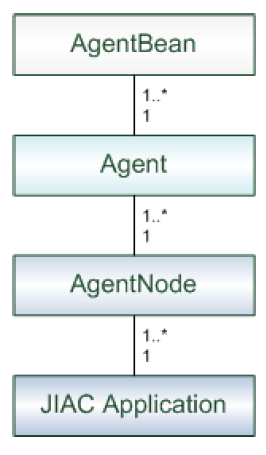
\includegraphics[width=0.25\textwidth]{images/jiac_basic.png}
		\caption{Jiac Basic concepts and their structural relationships \cite{JIACMAN10}}
	\label{fig:jiac_basic}
\end{figure}
An \textit{AgentNode} is a Java VM where the runtime infrastructure for agents, such as discovery services, white and yellow pages services, as well as communication infrastructure, are provided. A JIAC application might consists of multiple AgentNodes (distributed application). With the so-called AgentNodeBeans, one can extend the AgentNode with additional components.\\

Each AgentNode may run several \textit{Agents}. Agents provide services to other agents
and comprise lifecycle, execution cycle and a memory. An agent can use infrastructure
services in order to find other agents, to communicate to them and to use their services.
Skills and abilities of the agent can be extended by so-called AgentBeans.\\


\subsection{AgentBeans}
Beside using JADL, another mean to implement the functionality of an agent by implementing an agent bean attachable to the agent.
In most cases one can implement an agent bean simply by extending the class \texttt{AbstractAgentBean}. By doing this the new agent bean will have access to some useful fields such as :
\begin{itemize}
	\item \texttt{protected Log log} : a logger Instance that can be used to create log messages.
	\item \texttt{protected IAgent thisAgent} : Reference to the Agent object that can be used to perform operations on the agent
	\item \texttt{protected IMemory memory} : Reference to the Agents memory that can be used to store and retrieve data.
\end{itemize}

\textbf{Agent-Lifecycle}\\
An agent bean implements the interface \texttt{ILifeCycle} which provides operations to control the bean's state in accordance to the agent's lifecycle(see Figure \ref{fig:lifecycle}) by declaring the methods \texttt{init()}, \texttt{start()}, \texttt{stop()}, and \texttt{cleanup()}. These mehtods are implemented by the class \texttt{AbstractLifeCycle}, a super class of \texttt{AbstractAgentBean} which also provides the methods \texttt{doInit()}, \texttt{doStart()}, \texttt{doStop()}, and \texttt{doCleanup()} where we can hook up code that should be executed when the Lifecycle state changes, for example looking up needed actions, attaching SpaceObeserver to the agent's memory, etc.
\begin{figure}
	\centering
		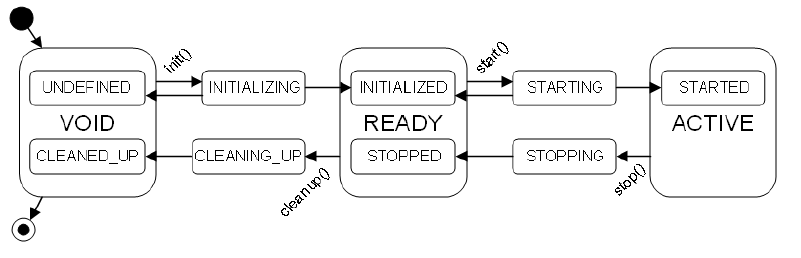
\includegraphics[width=1.00\textwidth]{images/lifecycle.png}
		\caption{Agent-Lifecycle \cite{JIACMAN10}}
		\label{fig:lifecycle}
\end{figure}

\textbf{Execution-Cycle}\\
By implementing the method \texttt{execute()}, we can tell the agent bean to do something periodically. This method is called by the agent's execution cycle, given that the execution intervall property is specified in the configuration file\footnote{Informations about the configuration file can be found in the jiac manual\cite{JIACMAN10}}, and while the agent is on the \textbf{started} state.\\

\textbf{Actions}\\
Agent beans can provide Actions. Actions are public methods that can be invoked by another bean and depending on the action's scope it can even be invoked by another agent. Therefore an action can be seen as a service. 
Using an Action normally includes two or three steps(the third one is optional):
\begin{enumerate}
	\item find the Action
	\item invoking the Action
	\item get the results
\end{enumerate}
The following Listing shows an example on how to use the send action provided by the \texttt{ICommunicationBean}:
\begin{lstlisting}[language = Java, caption = Using an Action]
Action sendAction = retrieveAction(ICommunicationBean.ACTION_SEND);//find action
[...]
invoke(sendAction, new Serializable{message, reciever})//invoke
\end{lstlisting}
The methods \textbf{\texttt{retrieveAction()}} and \textbf{\texttt{invoke()}} used in the above Listing are provided  by the \texttt{AbstractAgentBean}.\\

The simplest way to provide Actions is by extending the class \textbf{\texttt{AbstractMethodExposingBean}} (also an extension of \texttt{AbstractAgentBean}) and put the @Expose java annotation on the method that we want to expose as an action, as shown in the following listing:
\begin{lstlisting}[language = Java, caption = Providing an Action]
//static variable for the action name
public static final String ACTION_DOACTION = packagename.BeanName#doAction;
[...]
@Expose(name=ACTION_DOACTION, scope = ActionScope.GLOBAL)
public void doAction(){
[...]
}
\end{lstlisting}

\textbf{Memory and SpaceObserver}\\
The default implementation of the agent's memory is a simple tuple space that can hold any Java objects implementing the \textbf{\texttt{IFact}} interface (an extension to java.io.Serializeable). The memory provides the 4 methods to work on the space:\textit{ read, write, remove} and \textit{update}.

Each time a Bean calls an operation that modifies the memory, a SpaceEvent is fired. There are currently 4 different SpaceEvents that are fired:
\begin{itemize}
	\item \texttt{WriteCallEvent} - fired when a new object is written in the memory.
	\item \texttt{UpdateCallEvent} - fired when an object has been updated in memory.
	\item \texttt{RemoveCallEvent} - fired when an object is removed from the memory.
	\item \texttt{RemoveAllCallEvent} - fired when all objects are removed from the memory.
\end{itemize}

By using SpaceObserver, we can listen to these SpaceEvents and gets notification whenever a space event is being fired.
For example we can implement a space observer which will start a process when a message is being written in the memory (Listing \ref{list:SpaceObserver}). 
\begin{lstlisting}[language = Java, caption = A SpaceObserver, label = list:SpaceObserver]
SpaceObserver<IFact> observer = new SpaceObserver<IFact>(){
	public void notify(SpaceEvent<? extends IFact> event){
		if(event instanceof WriteCallEvent){
			doProcess(); //start process
		}
	}
};

memory.attach(observer);
\end{lstlisting}

To start recieving the SpaceEvents, we should attach the observer into the agent's memory (see line 9 of Listing \ref{list:SpaceObserver}). To stop recieving notifications on the SpaceEvents we can similarly use the \texttt{detach()} method.

\newpage
%======================================%
%                BPMN                  %
%======================================%
\section{BPMN(Business Process Modelling Notation)}
BPMN \cite{BPMN2} is a standard Notation for modelling business processes, initially published by the BPMI which is later adopted by the OMG(Object Management Group). A business process diagramm (as seen in Figure \ref{fig:bpmn_sampl}) can be compared to UML's activity diagram.\\
\begin{figure}[h]
	\centering
		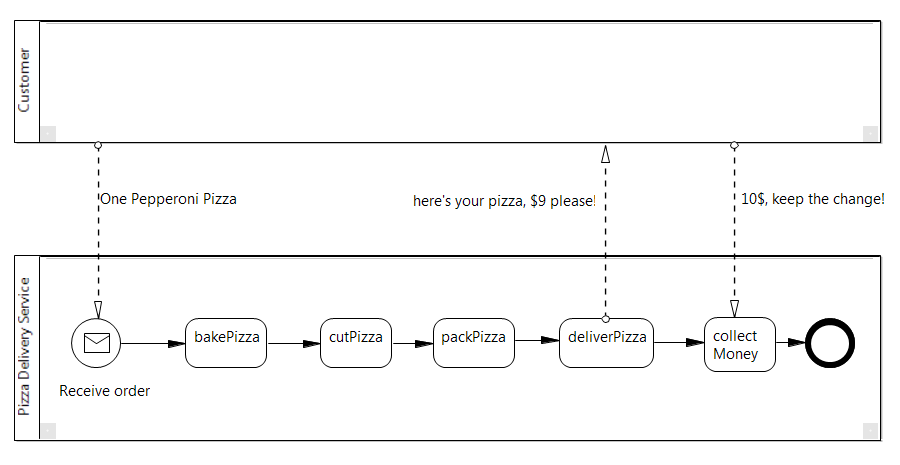
\includegraphics[width=0.90\textwidth]{images/bpmn_sampl.png}
	\caption{A simple Business Process Diagramm}
	\label{fig:bpmn_sampl}
\end{figure}

BPMN was made to provide a notation that is understandable by all business users, creating a bridge for the gap between the business process design and the process implementation. With the mapping of BPMN to Agents, we hope to be able to increase the spreading of the multi agent systems in the business world.


\subsection{Levels of Abstraction}
Besides providing an easy to read graphical notations, each BPMN elements are also equipped with additional attributes (so called properties), which are hidden from the diagram and provides the informations needed for automated code generation. The BPMN can be seen as having at least three levels of Abstraction:
\begin{enumerate}
	\item Basic Types - The diagram are made up of easily recognized graphical elements
	\item Subtypes - Each basic types can be further distinguished into subtypes with additional graphical elements such as icons that marks the type of an event's trigger.
	\item Properties - Each element has additional detailed informations that are hidden from the diagram, but contain informations needed for the transformation.
\end{enumerate}


\subsection{BPMN Elements}
BPMN elements can be categorized in five basic groups of elements\cite{BPMN2} :
\begin{itemize}
	\item Flow Objects
	\item Data
	\item Connecting Objects
	\item Swimlanes
	\item Artifacts
\end{itemize}
\textit{Flow Objects} includes Events, Activities and Gateways. These elements are the most important in BPMN, and they are held in a lane.\\

An \textit{Event} describes something that happens during the course of a process. It is divided into Start Event, Intermediate Event and End Event (see Figure \ref{fig:events}).\\
\begin{figure}[h]
	\centering
	
\includegraphics[width=0.25\textwidth]{images/events.png}
	\caption{BPMN Event types. From left to right: Start Event, Intermediate Event, End Event}
	\label{fig:events}
\end{figure}

BPMN Events are further divided into subtypes according to the type of the event's trigger (for start and intermediate events) or result (for end events). The event figure (see Figure \ref{fig:event_subtypes}) are drawn with different icon in the middle, according to the trigger.
\begin{figure}[htbp]
	\centering
	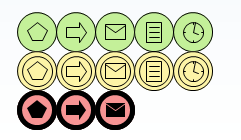
\includegraphics{images/event_types.png}
	\caption{Examples of event subtypes. From left to right: Multiple, Link, Message, Rule, Timer}
	\label{fig:event_subtypes}
\end{figure}

 
An \textit{Activity} describes something that is done during a process. It is divided into \textit{Tasks} which is an(Atomic Activities) and \textit{Sub Processes} (Composite Activities).\\
\begin{figure}[h]
\centering
\begin{tabular}{cc}
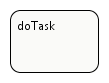
\includegraphics{images/mapping/task.png} & 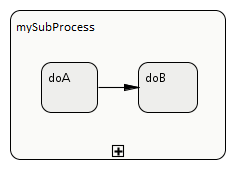
\includegraphics{images/mapping/subprocess.png}
\end{tabular}
\caption{Task(Left) and Subprocess}%
\label{fig:task+subprocess}%
\end{figure}

\newpage
\textit{Gateways} are used to define all kinds of splitting and merging behavior. It's semantics depends on the dimension of it's incoming and outgoing Sequence Flows. Gateways are divided into the following types (also see Figure \ref{fig:gateways}):\\
\begin{enumerate}
	\item Exclusive
	\item Event Based
	\item Inclusive
	\item Parallel
	\item Complex
\end{enumerate}



\begin{figure}[htbp]
	\centering
		
\includegraphics{images/gateways.png}
	\caption{Gateways - From left ro right: Exclusive, Event Based, Inclusive, Parallel, Complex}
	\label{fig:gateways}
\end{figure}



Data is representated by the four elements:
\begin{itemize}
	\item Data Objects
	\item Data Inputs
	\item Data Outputs
	\item Data Stores
\end{itemize}
\textit{Data Object} describes information that is needed by an activity or what they produce. It can represent a singular object or a collection of objects. \textit{Data Inputs} and \textit{Data Outputs} describe the same information for Processes. \textit{Data Stores} describe the location where information, that persists beyond the scope of a process are stored.\\\\
With \textit{ConnectingObjects}, FlowingObjects can be connected to each other or with other informations. There are 3 different kinds of Connecting Objects:
\begin{itemize}
	\item \textit{Sequence Flows} - represent Flow Control, used for connecting FlowObjects within a Pool in the order of execution.
	\item \textit{Message Flows} - represent Messages being exchanged exclusively between Pools.
	\item \textit{Associations} -  mainly used for documentation, in example between Flow Objects and a Text annotation.
\end{itemize}
\textit{Swimlanes} are divided into \textit{Pools} and \textit{Lanes}. Each Pool represents one Participant in the business process, while Lanes are used to partition a Pool, in example to model different Departments of an Institution. Figure \ref{fig:swimlane} shows a Pool with 2 Lanes.\\\\
\begin{figure}[htbp]
	\centering
		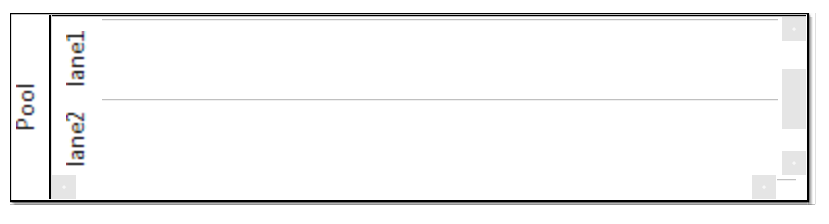
\includegraphics{images/swimlane.png}
	\caption{Pool with 2 Lanes}
	\label{fig:swimlane}
\end{figure}

\textit{Artifacts} are additional Information about the Process. It is mainly used for documentation purpose. The Current set of Artifacts includes:
\begin{itemize}
	\item Text Annotation
	\item Group
\end{itemize}


To provide a rough overview on how Agent technology can support the implementation of Business Processes let us take a look on this mapping example of BPMN elements to Agents. A Pool in a Business Process Diagram can represent an Agent, which are able to communicate with other agents (another pool) through messages (represented with the BPMN MessageFlows). Agents can react to Events. A detailed mapping needed for implementing the transformation will be discussed in chapter \ref{chap:mapping}

\newpage
%======================================%
%                VSDT                  %
%======================================%
\section{VSDT(Visual Service Design Tool)}
\label{sec:vsdt}
The VSDT is a CASE Tool, developed to support the idea of Process Oriented Agent Engineering, where Agents are designed by defining use cases and processes described with the BPMN. It's features include the BPMN editor, process structure view, model validation, import of existing web services, transformations to BPEL, and JIAC and many more. 
\begin{figure}[h]
	\centering
		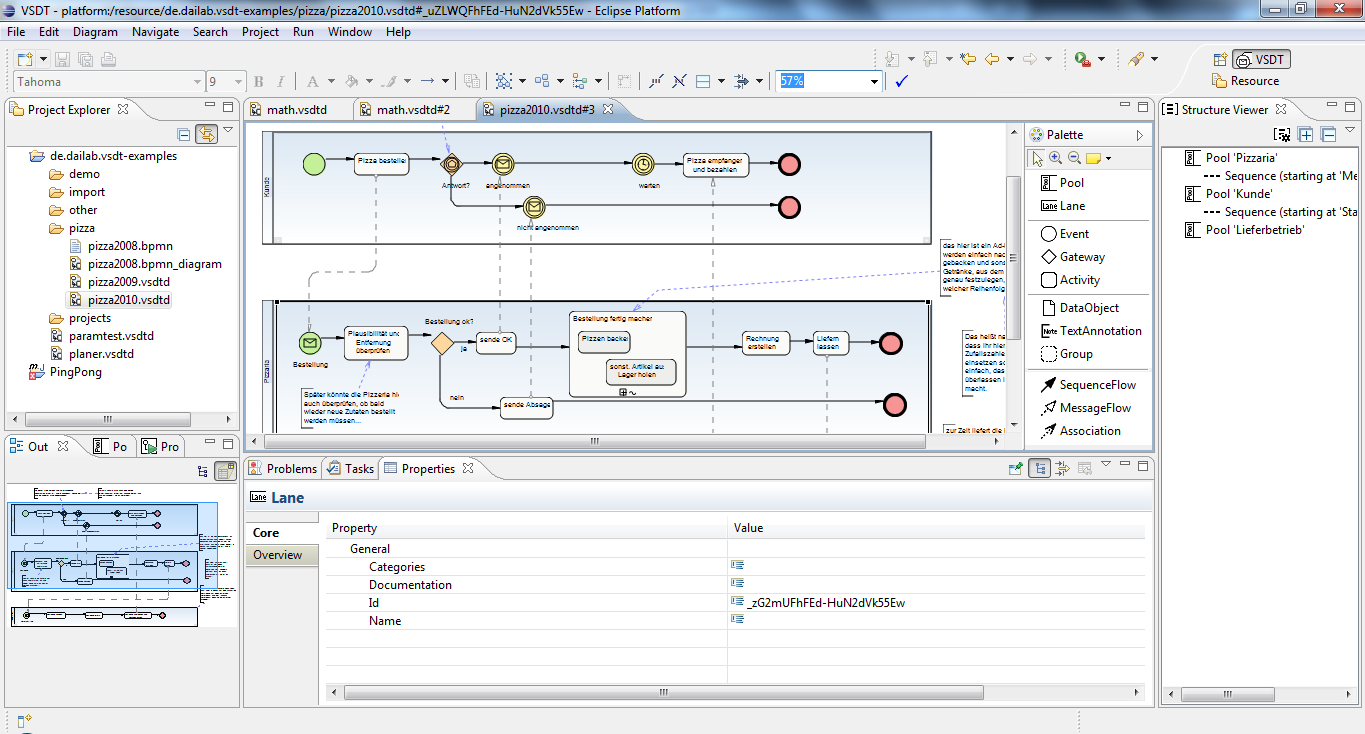
\includegraphics[width=0.90\textwidth]{images/vsdt_snapshot.png}
	\caption{VSDT - Editor View}
	\label{fig:VSDT}
\end{figure}

%========= The Editor =========%
\subsection{BPMN Editor}
The BPMN Editor in VSDT was created using eclipse's GMF (Graphical Modeling Framework). The editor enables us to create and modify business processes graphically. It also provides a properties view, where we can see and edit the additional properties of an element selected in the diagram. 

The VSDT was designed to support pure BPMN that is independent from any execution language\cite{TKAH08}. This means the standard editor doesn't support language specific features such as the validation of expression to be conform with the syntax of a specific language (such a validation can be implemented in the transformation). However, the editor can be enriched with plugins that for example provides a view with language specific funtionality.  


%========= Transformation Framework ===========%
\subsection{Transformation Framework}
Since it's initial development, VSDT's transformation framework is designed to be extensible and reuseable. This allows the development of a new transformation to be easier. For this purpose the transformation process is subdivided into several stages: 
\begin{enumerate}
	\item \textit{Validation}: Validate the input model.
	\item \textit{Normalisation}: Prepare the input model for transformation.
	\item \textit{Structure Mapping}: Convert the input model to a block-like structure.
	\item \textit{Element Mapping}: Perform the actual mapping, create target model.
	\item \textit{Clean Up}: Remove redundancies, improve readability, etc.
\end{enumerate}

Due to the fact that the validation, normalisation and structure mapping are mostly independent from the target language, the standard mapping provided for these stages are reuseable, which makes it possible to implement a new transformation by specifying the element mapping only. Figure \ref{fig:transform} shows the UML Class Diagram of the transformation famework with the example transformation to BPEL.
\begin{figure}[h]
	\centering
		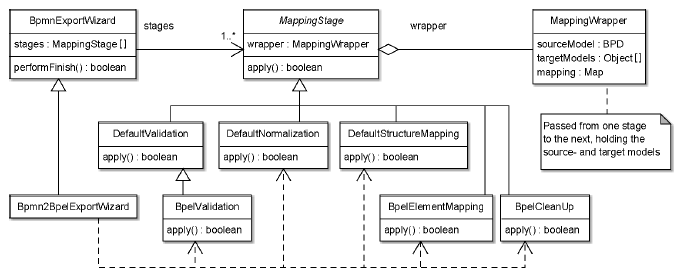
\includegraphics[width=0.90\textwidth]{images/transformation.png}
	\caption{Essential classes of the transformation framework, including the BPEL case.\cite{TK07}}
	\label{fig:transform}
\end{figure}

\newpage

%======================================%
%                 JET                  %
%======================================%
\section{JET(Java Emitter Templates)}
\textit{JET}\cite{JETWEB} is a code generating framework, developed as a part of the Eclipse Modelling Project \cite{EMPWEB}. Using the so-called templates, one can transform a model into various type of text, from a simple plain text up to text containing html, xml or java code. A naming convention exists for the JET-Template file according to the type of the generated text. For example the name of a template file generating a java code should end with \textit{.javajet}\\\\
The transformation process is done in two steps( see figure \ref{fig:jet_process} ). First, the JET-Builder will translate the template file into a Java class holding a generate method. Then we can create an instance of the template class and call it's generate method to get the result String which we can process further for example writing it into a file. 
\begin{figure}[h]
  \label{fig:jet_process}
	\centering
		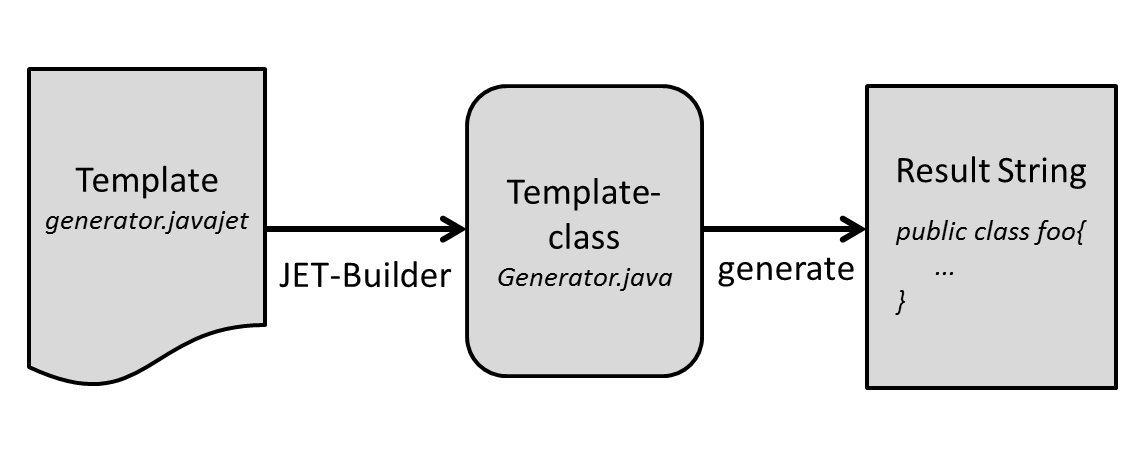
\includegraphics[width=1.0\textwidth]{images/jet_process.png}
	\caption{JET transformation steps.}
\end{figure}\\

\subsection{JET-Templates}
JET-Templates uses a JSP-like syntax which makes it easy to write and understand. There are three types of expression in JET-Syntax:
\begin{enumerate}
	\item \textbf{Directives} <\%\verb|@| \textit{directive \{attribute =  ''value''  \}*}\%>\\
	      Directives contains information for the JET-Engine. 
	      
	\item \textbf{Scriptlets} <\% \textit{scriplet} \%>\\
	      With Scriptlets we can use any java code fragment in the template. 
	      For example we can type cast the argument object into List:\\ 
	      \lstinline{<% List<String> studentlist = (List<String>) argument; %>} \\
	      These code fragments are executed at invocation time of the generate Method.
	      
	\item \textbf{Expressions} <\%= \textit{expression} \%>\\
	      An expression contains a java expression which will be executed at invocation time, and it's result will be added into the StringBuffer.
\end{enumerate}

A set of JET templates is called transformation. It is possible to build this transformation with a main template which acts as a visitor and runs through the model, and this main template will then use other templates which handle a specific element of the model. For example, in UML to Java transformation you can have special templates that handles the package, class, variables and methods.\\\\
The following listing shows a simple example of a JET-Template that generates an XML:
\begin{lstlisting}[caption = a simple JET-Template]
<% @ jet package="generator" imports="java.util.*" class="StudentListGenerator" %> 
<?xml version="1.0" encoding="UTF-8"?>
<% List<String> elementList = (List<String>) argument; %>
<class>
	 <% for (Iterator i = elementList.iterator(); i.hasNext(); ) { %>
     <student><%=i.next()%></student>
   <% } %>
</class>
\end{lstlisting}
A Jet-Template starts with the so called \textbf{jet-directive}. It contains informations for the JET-Builder, for example the name of the translated Java class(also called the template class), the package in which the template class should be placed into and a list of classes that should be imported by the template class.

In the first step, the JET-Builder will then translate this template into the Java Class generator.StudentListGenerator:
\begin{lstlisting}[caption = the translated Java-Class, language = Java]
package generator;
import java.util.*;

public class StudentListGenerator
{
  protected static String nl;
  public static synchronized StudentListGenerator create(String lineSeparator)
  {
    nl = lineSeparator;
    StudentListGenerator result = new StudentListGenerator();
    nl = null;
    return result;
  }
  public final String NL = nl == null ? (System.getProperties().getProperty("line.separator")) : nl;
  protected final String TEXT_1 = " " + NL + "<?xml version=\"1.0\" encoding=\"UTF-8\"?>";
  protected final String TEXT_2 = NL + "<class>" + NL + "\t ";
  protected final String TEXT_3 = NL + "     <student>";
  protected final String TEXT_4 = "</student>";
  protected final String TEXT_5 = NL + "</class>";
  public String generate(Object argument)
  {
    final StringBuffer stringBuffer = new StringBuffer();
    stringBuffer.append(TEXT_1);
     List<String> elementList = (List<String>) argument; 
    stringBuffer.append(TEXT_2);
     for (Iterator i = elementList.iterator(); i.hasNext(); ) { 
    stringBuffer.append(TEXT_3);
    stringBuffer.append(i.next());
    stringBuffer.append(TEXT_4);
     } 
    stringBuffer.append(TEXT_5);
    return stringBuffer.toString();
  }
}

\end{lstlisting}
The most interesting part of the java template class is the generate method. To get the text that should be generated, an instance of this class should be created and then we pass a list to the generate method, for example with the following code:
\begin{lstlisting}[caption = calling the generate method, language = Java]
  ...
  List<String> students = new ArrayList<String>();
  students.add("`Peter"');
  students.add("`John"');
  students.add("`Caroline"');
  
  StudentListGenerator generator = new StudentListGenerator();
  generator.generate(students);
\end{lstlisting}

, where the result of the transformation will be:
\begin{lstlisting}[caption = Result String of the transformation, language = xml]
	<class>
		<student>Peter</student>
		<student>John</student>
		<student>Caroline</student>
	</class>
\end{lstlisting}

\subsection{2 different JET-Versions}
There are currently 2 different JET-Versions in the Eclipse Modelling Project. The syntax and examples mentioned above correlate to the older Version of JET, which allows us to generate text with an Object as argument. In the template, the argument variable can be type casted into the class of our model. This JET-Version is effective if the model we want to generate the text from is a Java object. We get a String as a result which we can write into a File using the Java-IO or even Eclipse API.\\

In the updated version of JET, also called JET2, some workspace and java related "'tag-libraries"' are provided, enabling us to do the transformation without using the Java and Eclipse API. Unfortunately, in this Version the model has to be an xml-File.
Implementing the transformation of the BPMN directly from it's xml-Representation will be harder and the template will be confusing, therefore a decision has been made to implement the mapping using the existing transformation framework where an intermediate model class of the AgentBean will be created, and then transform this intermediate model into Java code using the older version of the JET Transformation.
More details on the implementation will be discussed in chapter \ref{chap:implementation}.

\subsection{New JET2 elements}
The enhanced version of JET comes with some new syntax elements such as:
\begin{itemize}
	\item Comments <\verb|--| \textit{Comment} \verb|--|>\\
	      Comments will be copied to the translated java class as a line comment, but they will have no influence on the transformation.
	\item Java Declaration <\%! ... \%>\\
	      Within the java declaration tag, the template may declare some java methods or variables.
	\item The @taglib directive <\%@taglib id=''...'' prefix=''...''\%>\\
	      With the @taglib directive, we can import an XML Tag Library or rename the taglibrary's namespace prefix.
	\item Custom xml tag\\
	   		JET2 templates may contain custom xml tags. JET2 comes with 4 standard tag libraries, and we can also define our own tag library.				
\end{itemize}

Out of the new elements, the custom XML tag is the most interesting since JET2 comes with 4 helpful standard tag libraries\cite{JET2TAGS}:
\begin{enumerate}
	\item Control tags\\
		    Contains control flow and data management tags. These tags will help us in visiting the input model where we will need to evaluate expression, perform loops,  iterate through a certain set of elements and read or write some informations in the input. 
	\item Workspace tags\\
			  Contains a set of library that performs operations against the eclipse workspace (for example for creating a file in an existing eclipse Project). 
	\item Java tags\\
				Contains tags useful for generating java codes such as creating java packages and classes, managing imports etc.
	\item Format tags\\
		    Standard tags for formatting text. 
\end{enumerate}

